\documentclass[e4_tp1_main.tex]{subfiles}

\begin{document}
	
	\section{Ejercicio 4}
	
	\subsection{Modo discontinuo}
	En esta sección se muestran las diversas curvas ya calculadas en las secciones anteriores pero trabajando en modo de conducción discontinua (DCM). Para ello, es necesario calcular la corriente de boundary para saber el valor de corriente a partir del cual se comenzará a trabajar en modo discontinuo.
	
	Habiendo calculado previamente el valor de $\Delta I_{L}$ y sabiendo que $I_{OB}=\frac{\Delta I_{L}}{2}$ se obtiene que:
	
	\begin{equation}
	I_{OB}=0.11A    
	\end{equation}
	
	Sabiendo el valor de $I_{OB}$ podemos obtener la resistencia mínima para que la fuente trabaje en modo de conducción discontinua, a saber:
	
	\begin{equation}
	R_{min}=\frac{V_O}{I_{OB}}=33.63\Omega
	\end{equation}
	
	Sabiendo esto, para que los efectos del modo de conducción discontinua puedan ser percibidos se eligió una resistencia de $150\Omega$.
	
	A continuación se presentan las distintas señales solicitadas.
	
	\subsubsection{Señal de disparo y conmutación de la llave}
	A continuación se muestran la señal de disparo junto con las señales de conmutación de la llave, a saber: tensión de gate, tensión drain-source y corriente de drain.
	
	\begin{figure}[H]
		\centering
		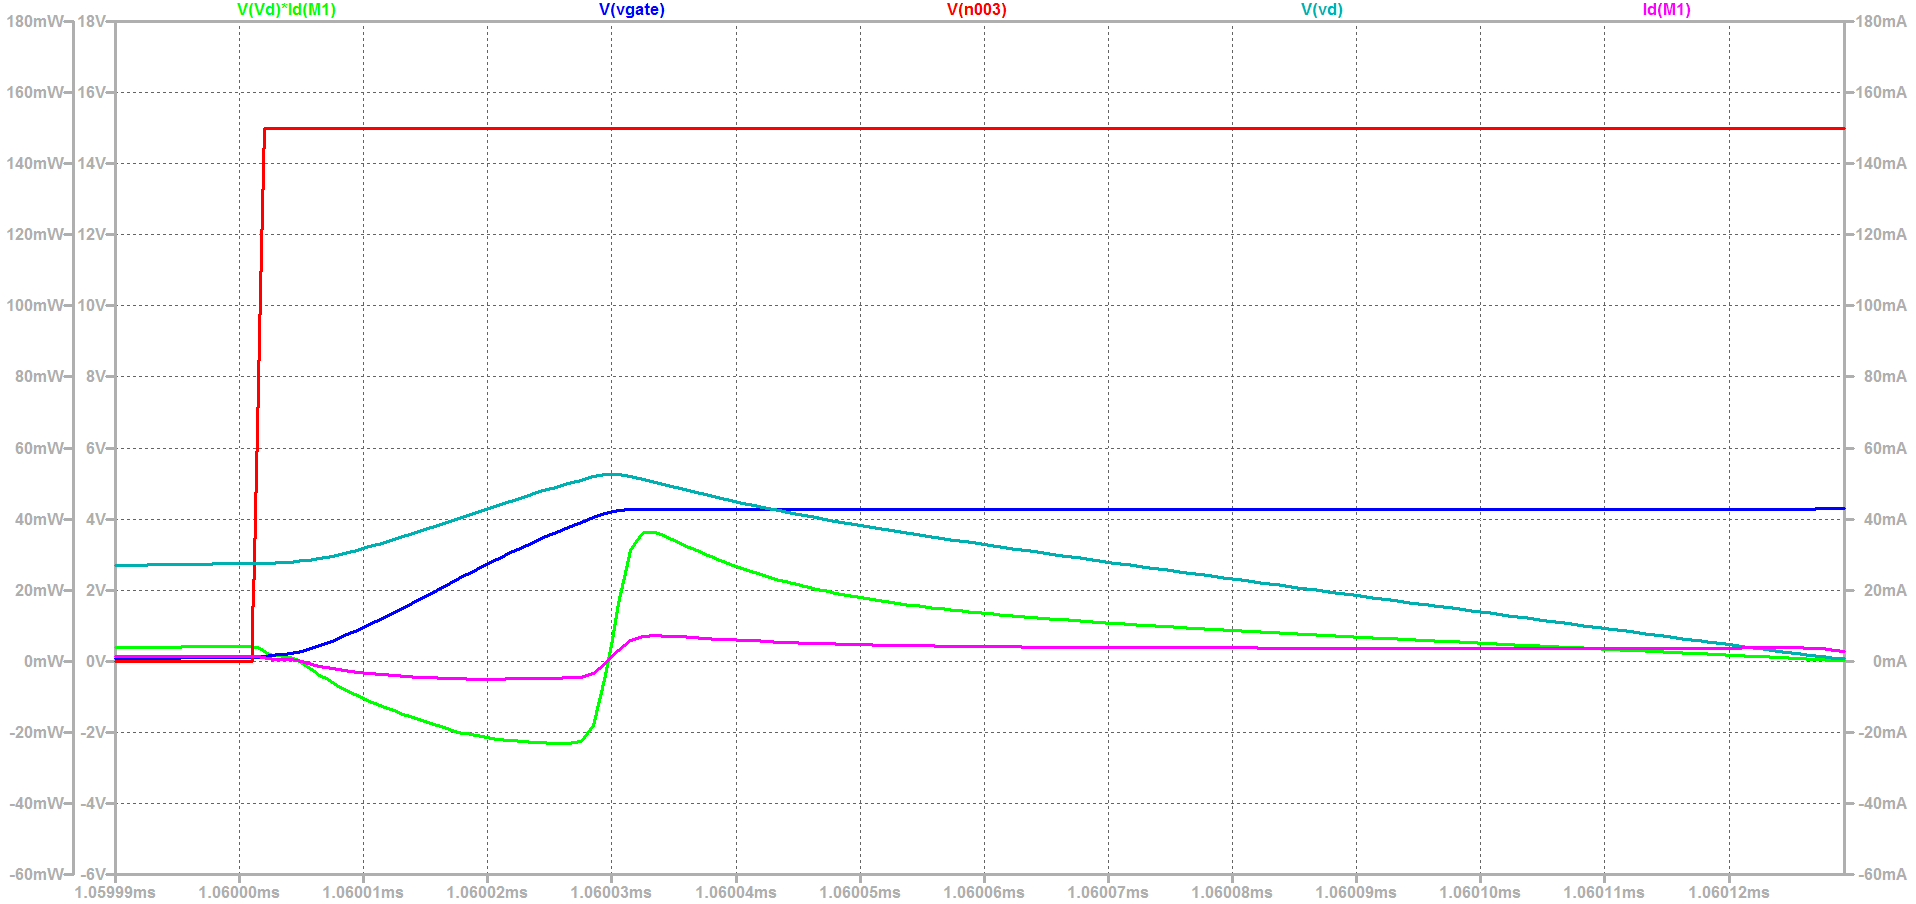
\includegraphics[width=0.8\textwidth]{images/ej4/fig1.png}
		\caption{Encendido de la llave}
		\label{fig:my_label}
	\end{figure}
	
	Al observar el encendido de la llave trabajando en modo discontinuo se puede ver que la corriente de drain crece al ritmo de la corriente del inductor desde el momento inicial. Esto se debe a que la corriente del inductor es cero ya que el mismo se encontraba descargado al momento de encender la llave. De hecho, por este motivo, el crecimiento resulta despreciable durante la caída de tensión de drain-source, lo cual resulta en una pérdida de potencia prácticamente igual a cero, que se calculará más adelante. En el caso del continuo, la corriente de drain crecía rápidamente para igualar a la del inductor, resultando en una mayor pérdida de potencia dado el producto $V_{DS}*I_d$, que también se calculará al realizar el estudio de pérdidas en la conmutación.
	
	\begin{figure}[H]
		\centering
		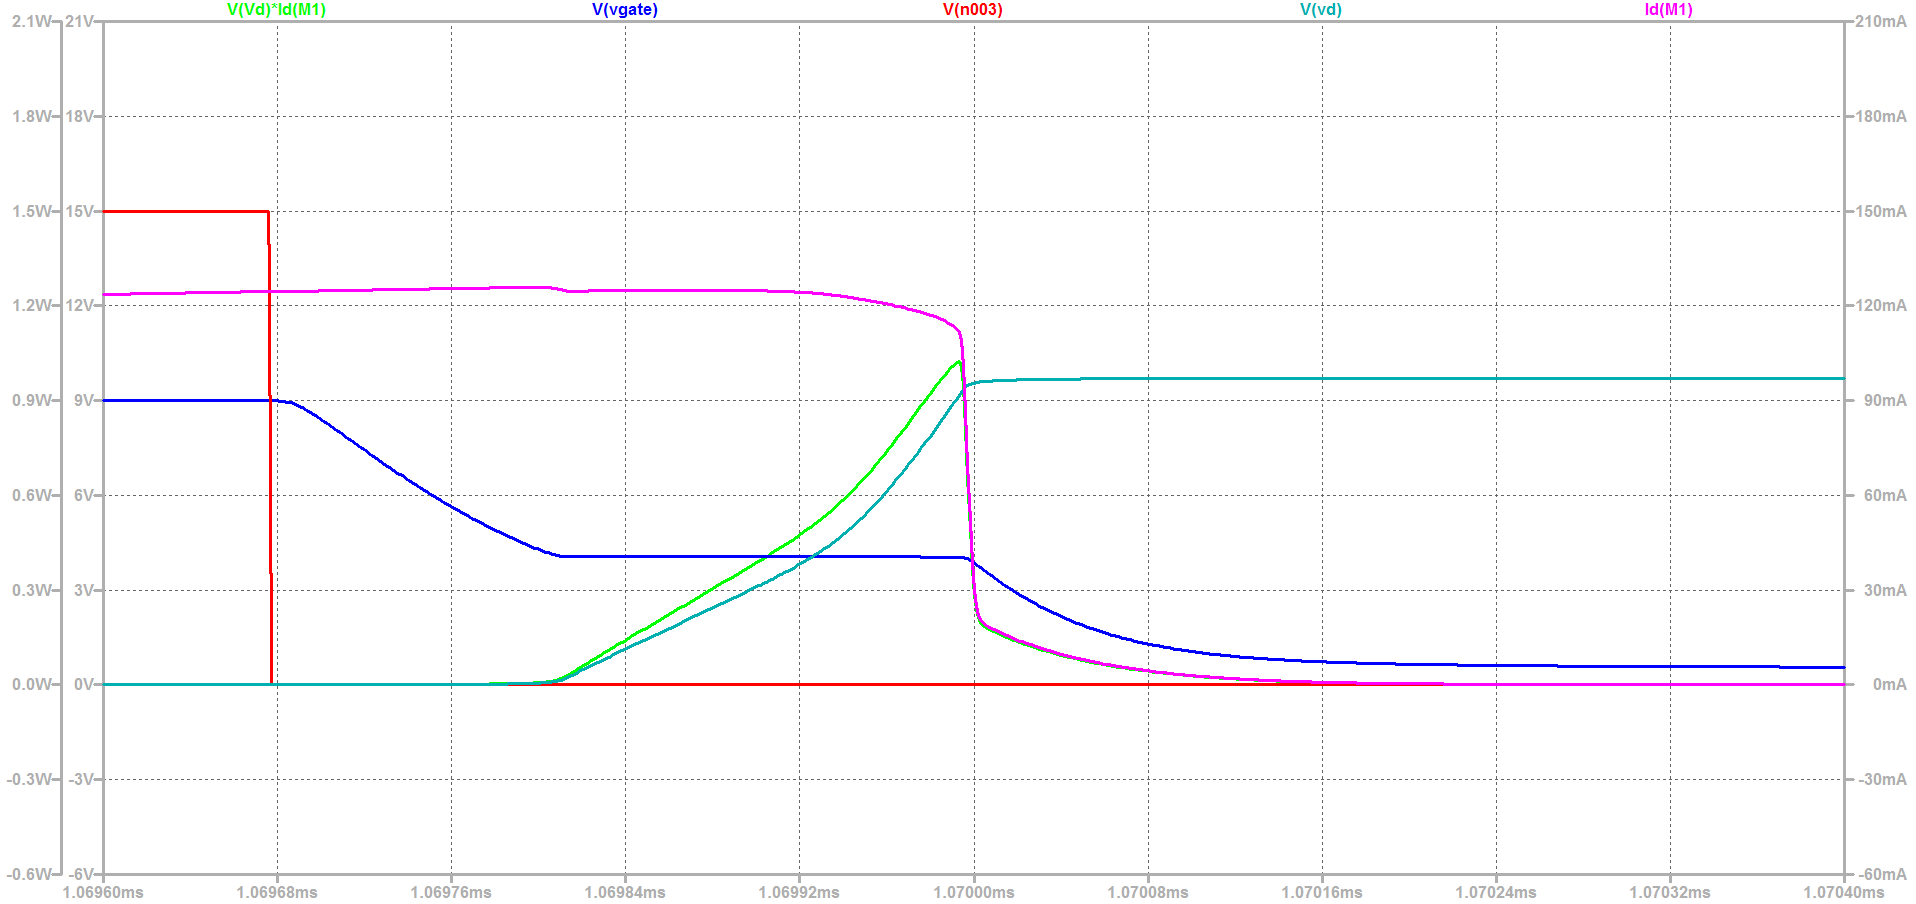
\includegraphics[width=0.8\textwidth]{images/ej4/fig2.png}
		\caption{Apagado de la llave}
		\label{fig:my_label}
		
	\end{figure}
	
	En el apagado de la llave no ocurre lo mismo que en el encendido ya que la corriente de drain estará regida por la corriente del inductor, la cual no será nula en este punto. No habrá una diferencia significativa en las formas de onda entre el modo discontinuo y el continuo, solamente se podrá observar una diferencia en las magnitudes de la corriente del drain, lo cual  se podrá apreciar en la potencia de pérdida instantánea. 
	
	De este análisis podemos determinar que en el caso del apagado no se podrá determinar a priori cuál de los dos modos perderá más potencia por apagar la llave, ya que depende de las condiciones del circuito. En cambio, en el encendido, el modo discontinuo siempre contará con una pérdida de potencia prácticamente nula.
	
	
	\subsubsection{Corriente en el inductor y en el diodo}
	A continuación se muestra el gráfico correspondiente a las corrientes del inductor y del diodo trabajando en modo discontinuo:
	
	\begin{figure}[H]
		\centering
		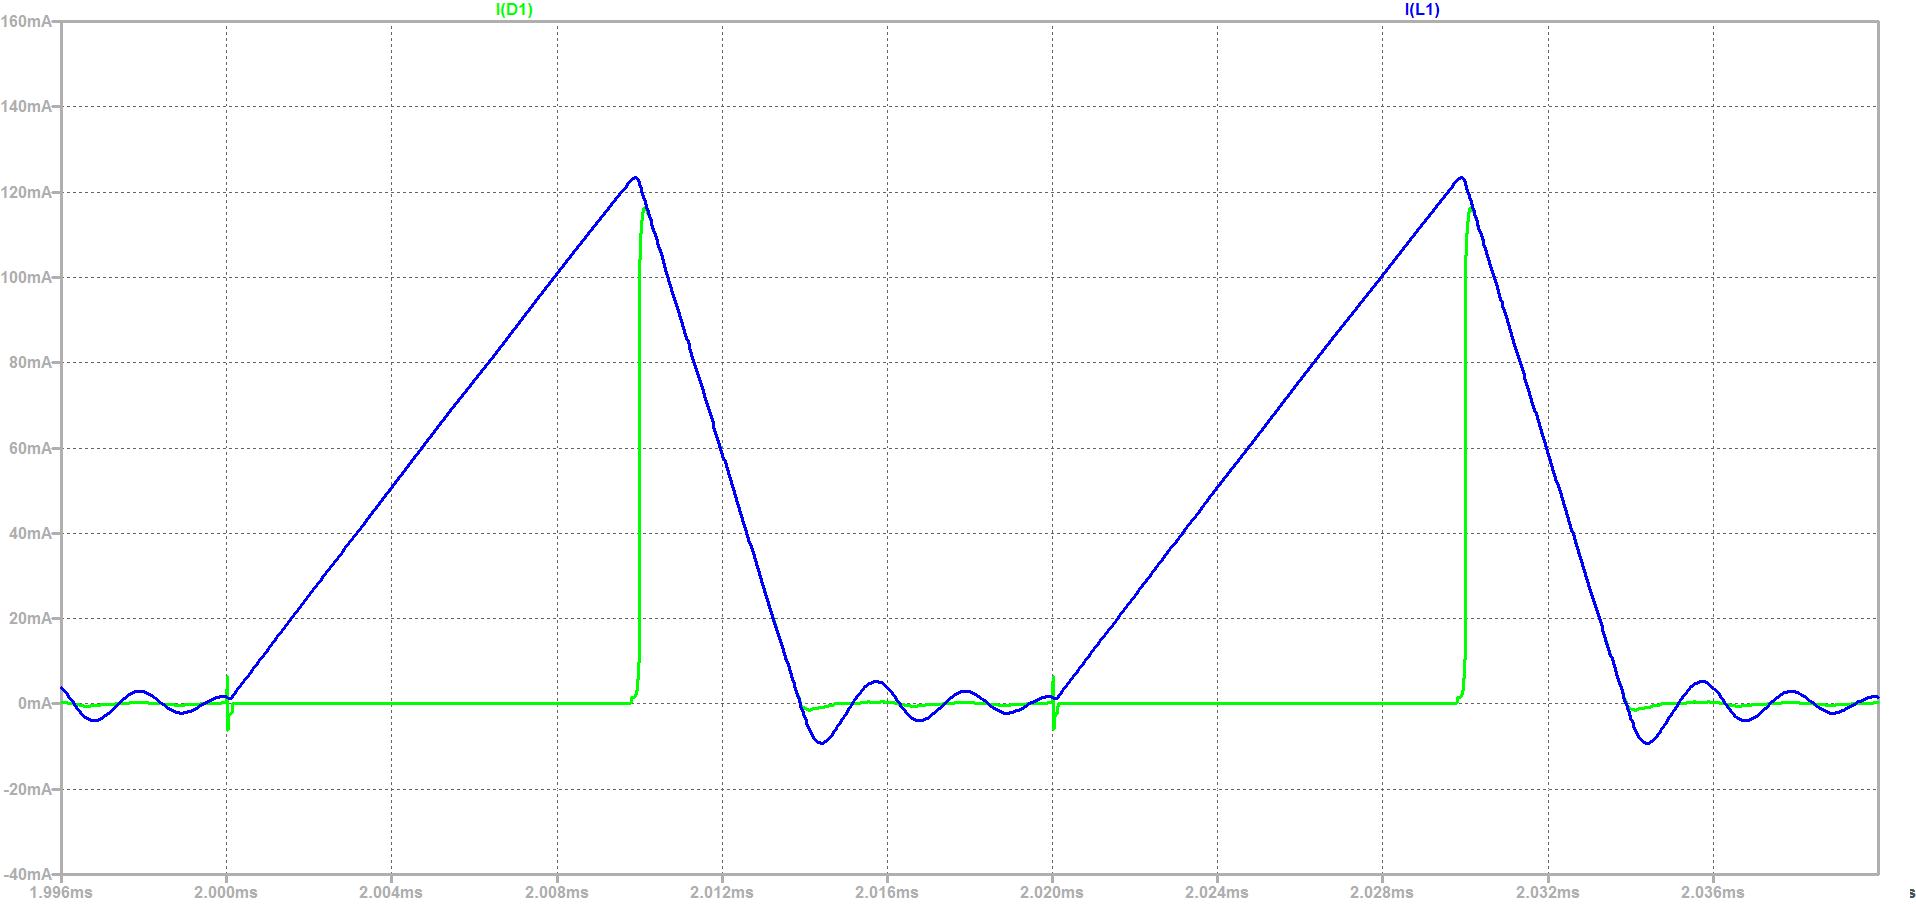
\includegraphics[width=0.72\textwidth]{images/ej4/fig3.png}
		\caption{Corriente en el inductor y en el diodo}
		\label{fig:my_label}
	\end{figure}
	
	En la figura se puede observar que al igual que en modo continuo el diodo sigue la corriente del inductor durante el tiempo en el que la llave se encuentra apagada. Sin embargo, al comparar con el caso continuo, se hace visible la diferencia entre el tiempo de crecimiento de la corriente respecto del de caída de la misma. El hecho de que el crecimiento de la corriente no sea simétrico respecto de la caída hace que el inductor se descargue antes de la próxima conmutación de la llave, generando así que la misma llegue hasta cero, haciendo que el circuito trabaje en modo discontinuo.
	
	Al llegar al valor de corriente igual a cero, se observa una oscilación de la misma a modo de "ringing" o resonancia. Esto se debe a los intercambios de energía producidos durante ese tiempo en el cual se genera un punto de alta impedancia producido por la llave abierta, el diodo qu se encuentra en inversa, y la resistencia propia con el capacitor cargado en paralelo, los cuales en conjunto con el inductor dan lugar también a un RLC resonante.
	
	\subsubsection{Tensión en el inductor}
	A continuación se muestra el gráfico correspondiente a la tensión del inductor y en modo discontinuo:
	\begin{figure}[H]
		\centering
		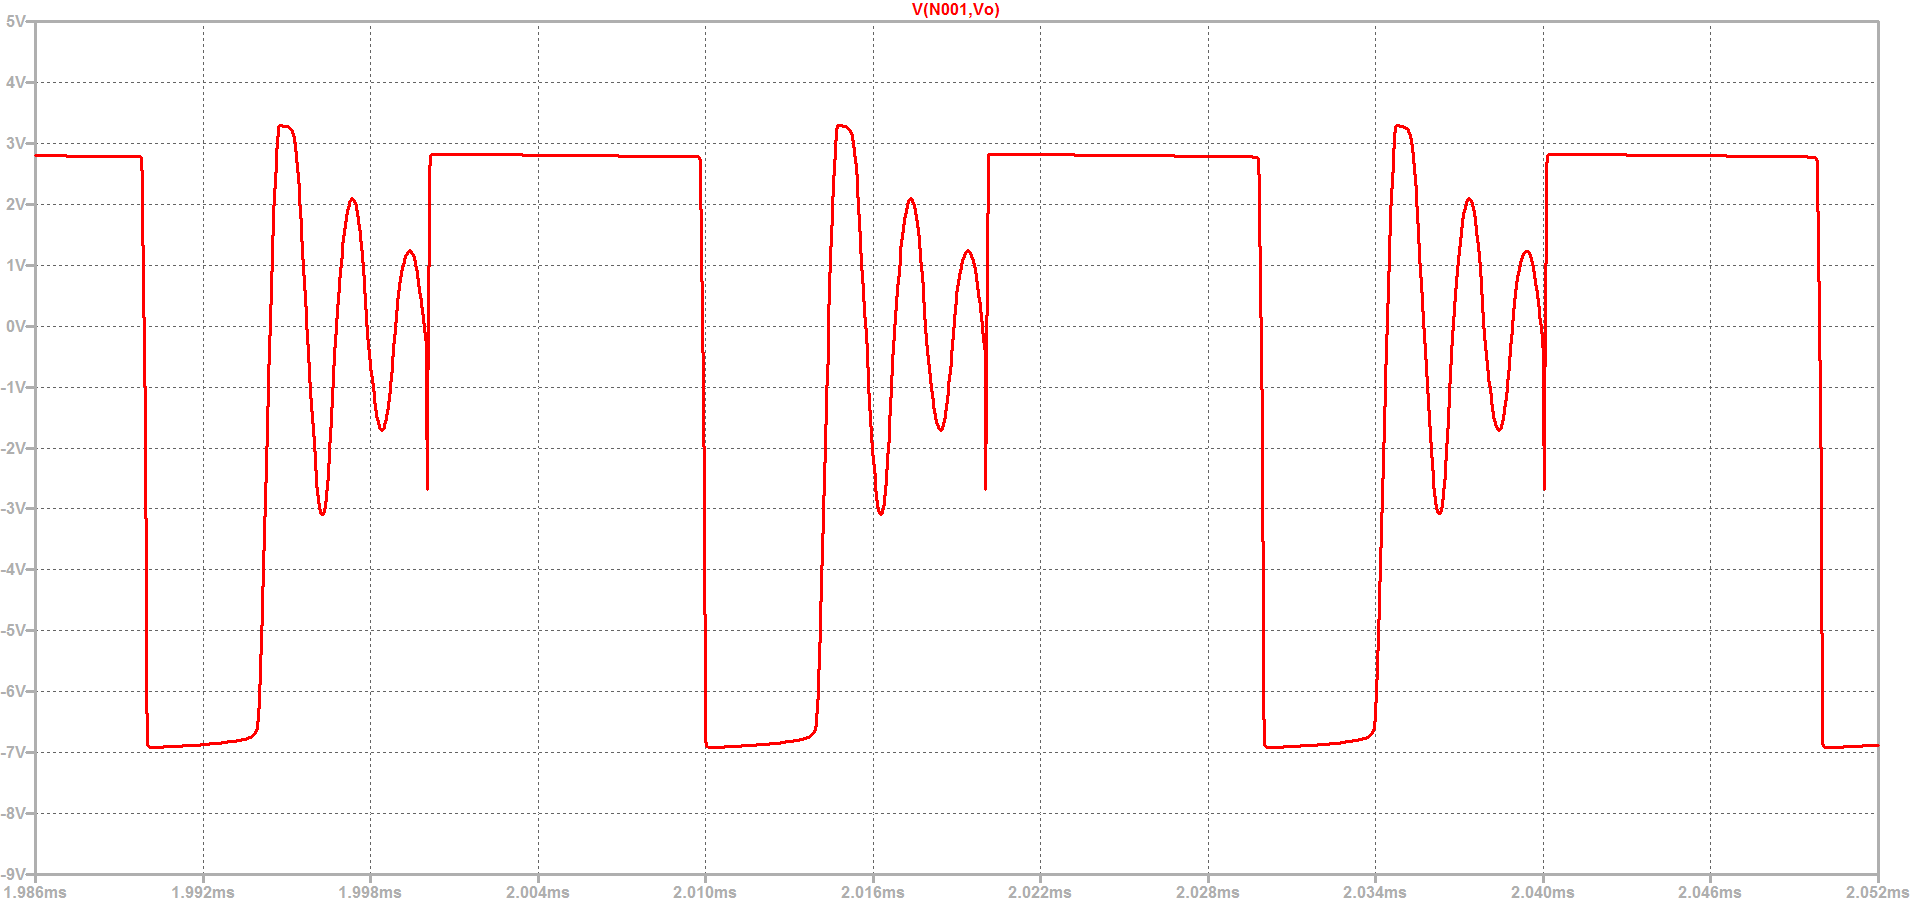
\includegraphics[width=0.8\textwidth]{images/ej4/fig4.png}
		\caption{Tensión en el inductor}
		\label{fig:my_label}
		
		En esta figura se puede observar claramente los tiempos de carga y descarga del inductor, siendo el tiempo de  carga mucho mayor al de descarga correspondiente. Aquí también se puede vislumbrar que el tiempo en el cual la llave permanece encendida es el mismo que el que la llave permanece apagada. Sin embargo, la tensión no se mantiene constante en todo el intervalo de tiempo en el que la llave está apagada debido al "ringing" explicado previamente en la corriente del inductor.
		
	\end{figure}
	\subsection{Pérdidas en modo continuo y discontinuo}
	A continuación se procede a calcular las pérdidas de pontencia por conmutación en la llave tanto en el modo continuo como en el discontinuo. 
	
	Para poder hacer esto se utilizó la herramienta de integración de LTspice para poder obtener la energía perdida en el intervalo de tiempo de cada conmutación (ON/OFF). Para poder definir un intervalo de tiempo adecuado, es decir, el intervalo en el cual el producto $V_{DS}\times I_d\neq 0$, se consideraró cero a aquellos valores inferiores a $50mV$ y $0.5\mu A$.
	
	\subsubsection{Pérdidas en modo continuo}
	De los gráficos de conmutación de la llave en modo continuo se obtuvo que:
	
	En el encendido:
	\[t_{ri}+t_{fv}=249.5ns\]
	
	\[W_{c_{ON}}=249.67nJ\]
	
	\[P_{c_{ON}}=F_s\times W_{c_ON}=12.4835mW\]
	
	En el apagado:
	\[t_{rv}+t_{fi}=480ns\]
	
	\[W_{c_{OFF}}=354.19nJ \]
	
	\[P_{c_{OFF}}=F_s\times W_{c_{OFF}}=17.7095mW\]
	
	Entonces la potencia total de pérdida por conmutación equivale a:
	\[P_c=F_s(W_{c_{ON}}+W_{c_{OFF}})=30.193mW\]
	
	Que porcentualmente representa:
	\[P_{c\%}=\frac{P_c}{P_c+V_OI_O}\]
	
	Y sabiendo que:
	\[V_O=3.758V\]
	\[I_O=0.3758A\]
	
	Finalmente resulta:
	
	
	\[P_{c\%}=2.0931\%\]
	
	
	
	\subsubsection{Pérdidas en modo discontinuo}
	De los gráficos de conmutación de la llave en modo discontinuo se obtuvo que:
	
	En el encendido:
	\[t_{ri}+t_{fv}=127.7ns\]
	
	
	
	\[W_{c_{ON}}=0.71222nJ\]
	
	
	
	\[P_{c_{ON}}=F_s\times W_{c_{ON}}=0.035611mW\]
	
	
	En el apagado:
	
	\[t_{rv}+t_{fi}=388.7ns\]
	
	
	
	\[W_{c_{OFF}}=95.342nJ\]
	
	\[P_{c_{OFF}}=F_s\times W_{c_{OFF}}=4.7671mW\]
	
	Entonces la potencia total de pérdida por conmutación equivale a:
	\[P_c=F_s(W_{c_{ON}}+W_{c_{OFF}})=4.8027mW\]
	
	Que porcentualmente representa:
	\[P_{c\%}=\frac{P_c}{P_c+V_OI_O}\]
	
	Y sabiendo que:
	\[V_O=6.24V\]
	\[I_O=0.041A\]
	
	Finalmente resulta:
	
	\[P_{c\%}=1.842\%\]
	
	\subsubsection{Conclusiones}
	De los resultados obtenidos, por un lado, se puede destacar el hecho de que la potencia perdida en el encendido de la llave en el modo discontinuo  efectivamente es cercana a cero, comparada con todas las demás. Además, se pudo ver que si bien la potencia total de pérdida por conmutación fue mayor en el modo continuo, la pérdida porcentual no lo fue tanto. Esto se debe a que al trabajar en modo discontinuo se alteran tanto la tensión como la corriente de salida de la fuente, provocando que disminuzca la potencia entregada a la carga y, por ende, la potencia total entregada por la fuente. 
	
	Finalmente podemos concluir que no hay un modo de trabajo que tenga menos pérdidas de forma previsible y que dependerá de las características de la fuente con la que se esté trabajando. 
	
	Además notar que, al no contar con un controlador, no se puede regular el duty cycle de la señal de disparo de forma tal que se pueda obtener la salida de tensión deseada, a pesar de estar en modo discontinuo. Esto implica que si contásemos con un control, de forma tal de obtener la misma tensión en la carga, habría que corroborar nuevamente qué modo presenta mayores pérdidas.
	
\end{document}

\begin{equation}

\end{equation}	

\end{document}
